\documentclass[aspectratio=169,11pt]{beamer}

\usetheme{Madrid}
\usecolortheme{default}
\usepackage{amsmath}
\usepackage{booktabs}
\usepackage{graphicx}
\usepackage{hyperref}
\usepackage{xcolor}

\graphicspath{{../assets/}}
\setbeamertemplate{navigation symbols}{}
\setbeamertemplate{caption}[numbered]
\definecolor{Ink}{HTML}{1F2937}
\definecolor{Accent}{HTML}{0F766E}
\setbeamercolor{title}{fg=Ink}
\setbeamercolor{frametitle}{fg=Ink}
\setbeamercolor{structure}{fg=Accent}

\title[Experiments]{Experiments\\Reproduction of High-Dimensional MSWD Testing}
\author{MSWD Bootstrapping Reproduction}
\date{\today}

\begin{document}
\section{Experiments}

\begin{frame}[plain]
  \titlepage
\end{frame}

\begin{frame}{How the paper connects the experiments}
\begin{itemize}
  \item Goal: test \(H_0:P=Q\) versus \(H_1:P\neq Q\) in high dimension.
  \item Core statistic: maximize one-dimensional Wasserstein distance over sparse directions.
  \[
  T_n=\left(\frac{n_1n_2}{n_1+n_2}\right)^{1/2}
  \sup_{v\in V_{0,s}} W_1(v^\top X,v^\top Y).
  \]
  \item Decision: reject if observed \(T_n\) exceeds the bootstrap \(1-\alpha\) quantile.
  \item SCI: the same bootstrap construction also localizes marginal genes and GO-term subsets.
\end{itemize}
\end{frame}

\begin{frame}{Three experiments and their roles}
\begin{tabular}{p{0.22\linewidth}p{0.34\linewidth}p{0.34\linewidth}}
\toprule
Experiment & Question & Output \\
\midrule
Model A comparison & Does MSWD have a power advantage in the core simulation? & Empirical rejection curves from 50 runs \\
MSWD-only bootstrap & How does the statistic compare with its null distribution? & Observed \(T_n\), threshold, p-value \\
GBM real data & Are LGG and GBM methylation distributions different, and where? & Global test, 138 genes, 7 GO terms \\
\bottomrule
\end{tabular}
\end{frame}

\begin{frame}{Experiment 1 setup: Model A, first 50 Monte Carlo runs}
\begin{itemize}
  \item Model: \(X\sim N(0_p,\Sigma)\), \(Y\sim N(\mu,\Sigma)\).
  \item Covariance: \(\Sigma_{ij}=0.5^{|i-j|}\).
  \item Decaying mean shift: \(\mu_j=0.8\beta j^{-3}\).
  \item Parameters: \(n_1=n_2=250\), \(p=500\), \(\alpha=0.05\).
  \item Signal grid: \(\beta=0,0.2,0.4,0.6,0.8,1.0\).
  \item Reported as 50 complete runs per \(\beta\); Proposed bootstrap \(B=300\).
  \item Comparators: MMD-G, ED$_2$, BG, PW; MMD-L is not recoverable from logs.
\end{itemize}
\end{frame}

\begin{frame}{Experiment 1 result: Proposed gains power fastest}
\begin{center}
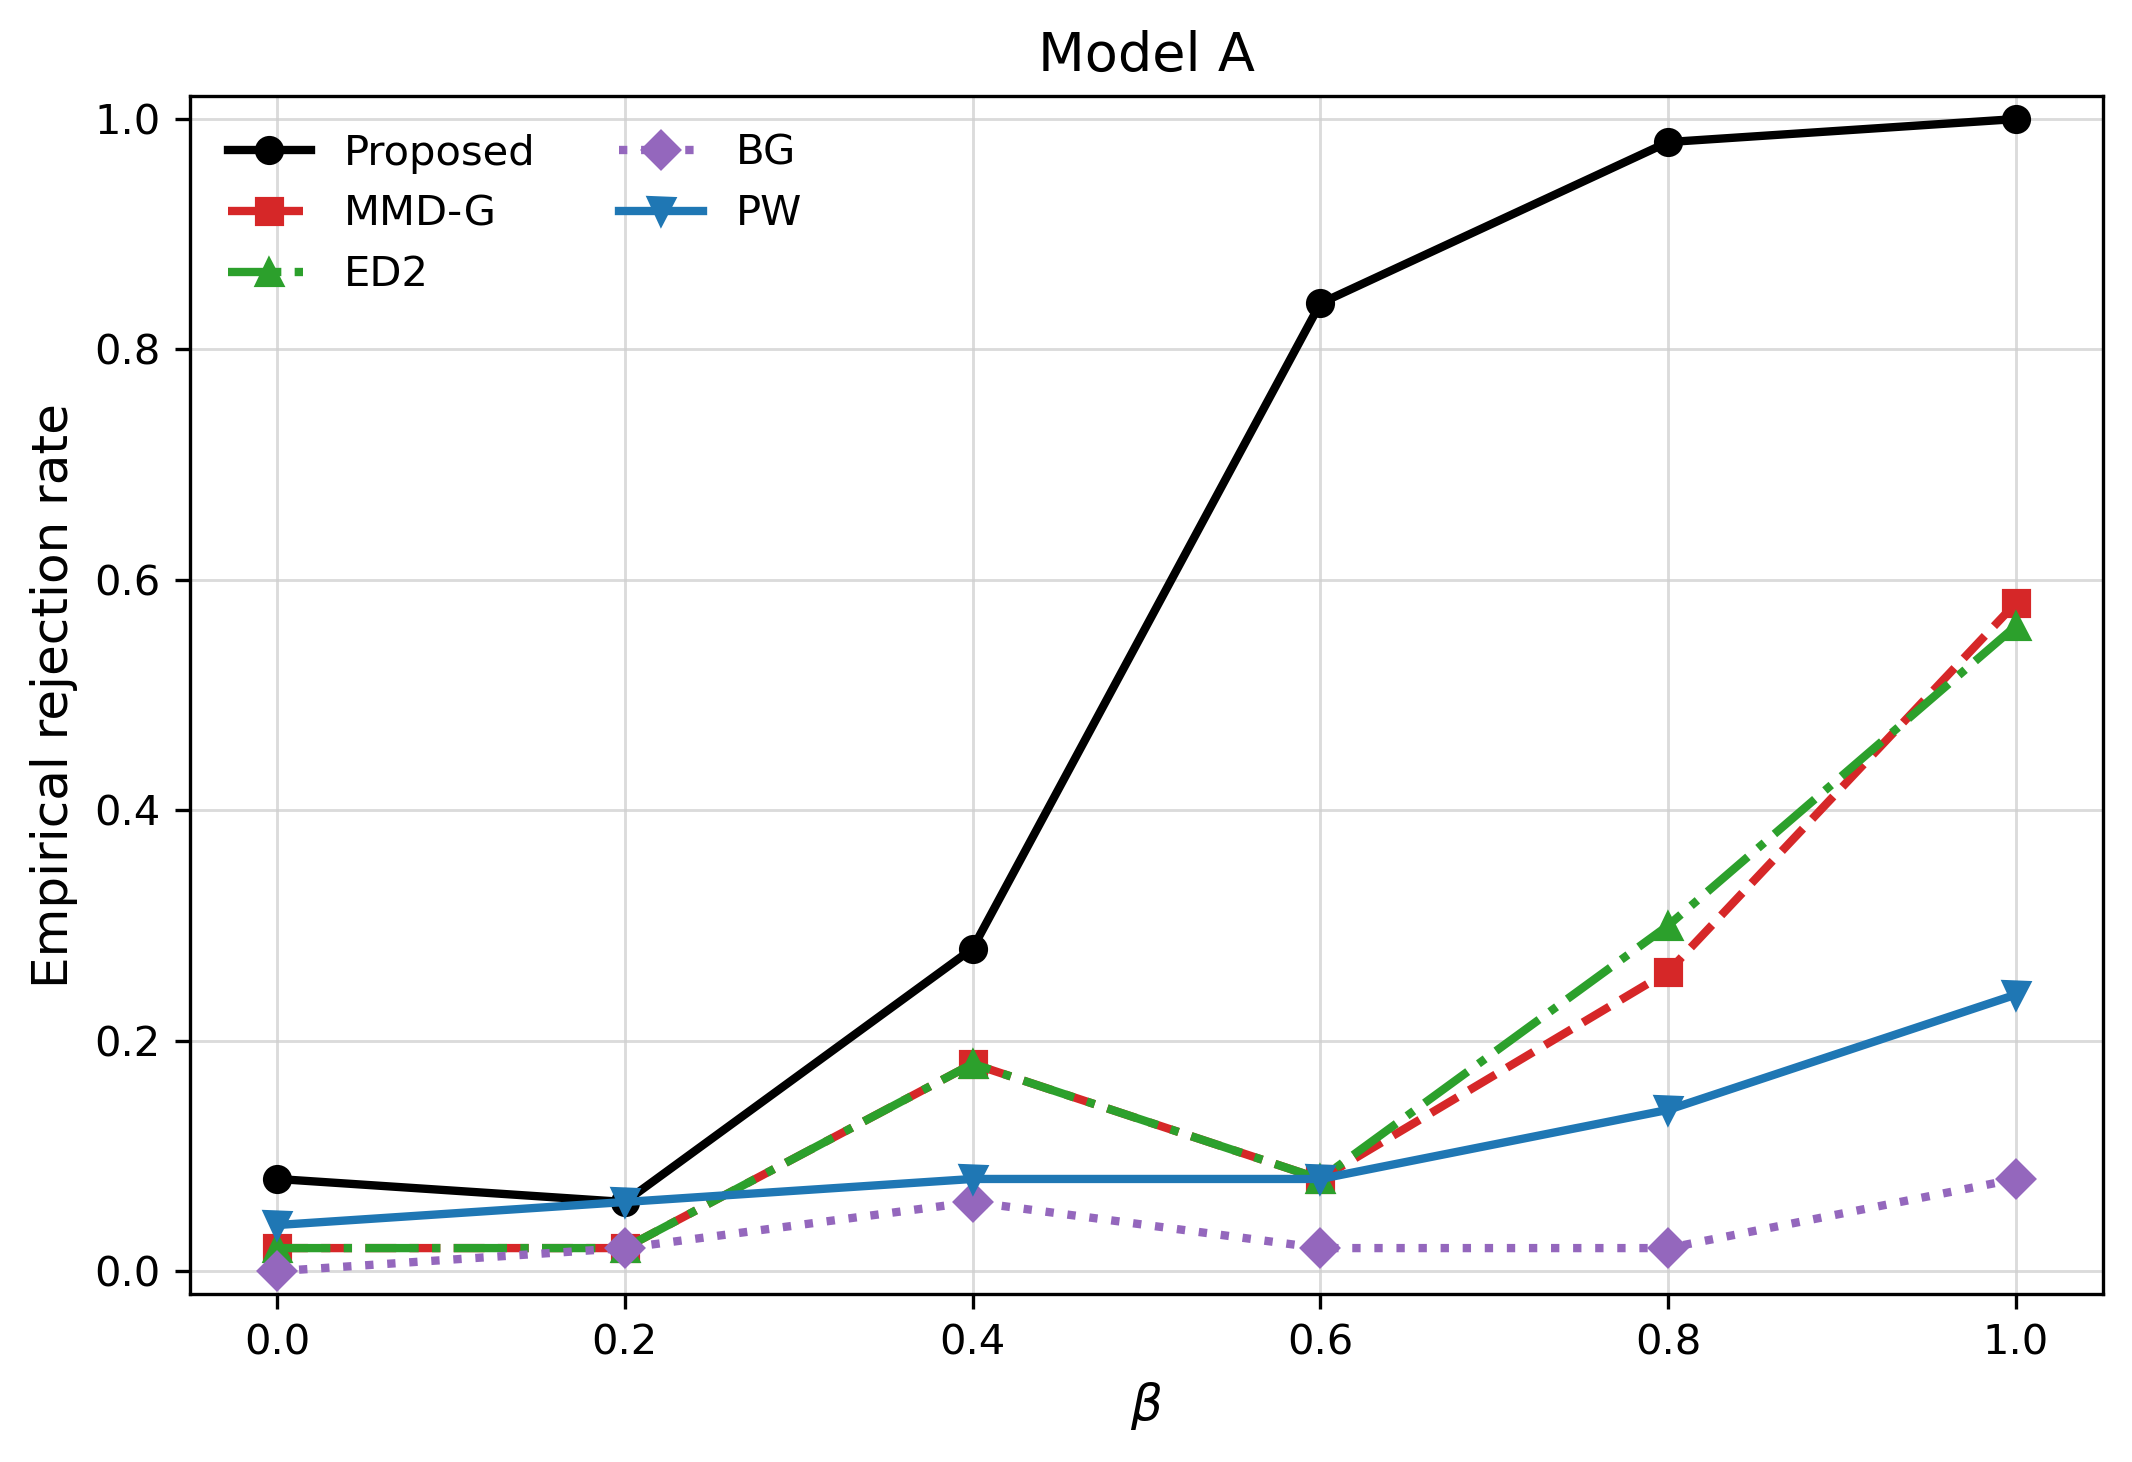
\includegraphics[width=0.82\linewidth,height=0.74\textheight,keepaspectratio]{fig1.png}
\end{center}
\end{frame}

\begin{frame}{Experiment 1 interpretation}
\small
\begin{tabular}{cccccc}
\toprule
\(\beta\) & Proposed & MMD-G & ED$_2$ & BG & PW \\
\midrule
0.0 & 0.08 & 0.02 & 0.02 & 0.00 & 0.04 \\
0.4 & 0.28 & 0.18 & 0.18 & 0.06 & 0.08 \\
0.6 & 0.84 & 0.08 & 0.08 & 0.02 & 0.08 \\
0.8 & 0.98 & 0.26 & 0.30 & 0.02 & 0.14 \\
1.0 & 1.00 & 0.58 & 0.56 & 0.08 & 0.24 \\
\bottomrule
\end{tabular}

\vspace{0.25cm}
\begin{itemize}
  \item At \(\beta=0\), size is about 0.08 for Proposed, plausible with 50 runs.
  \item From \(\beta=0.6\), Proposed separates sharply, matching the paper's message on sparse decaying signals.
\end{itemize}
\end{frame}

\begin{frame}{Experiment 2 setup: MSWD-only bootstrap}
\begin{itemize}
  \item One Model A data set is generated for each \(\beta\).
  \item Each data set receives \(B=500\) bootstrap replications.
  \item This is not a power experiment; it visualizes the test decision.
  \item Decision rule: observed \(T_n\) greater than the 95\% bootstrap threshold.
  \item Parameters: \(n_1=n_2=250\), \(p=500\), \(\alpha=0.05\).
\end{itemize}
\end{frame}

\begin{frame}{Experiment 2 result: strong signals exceed the threshold}
\begin{center}
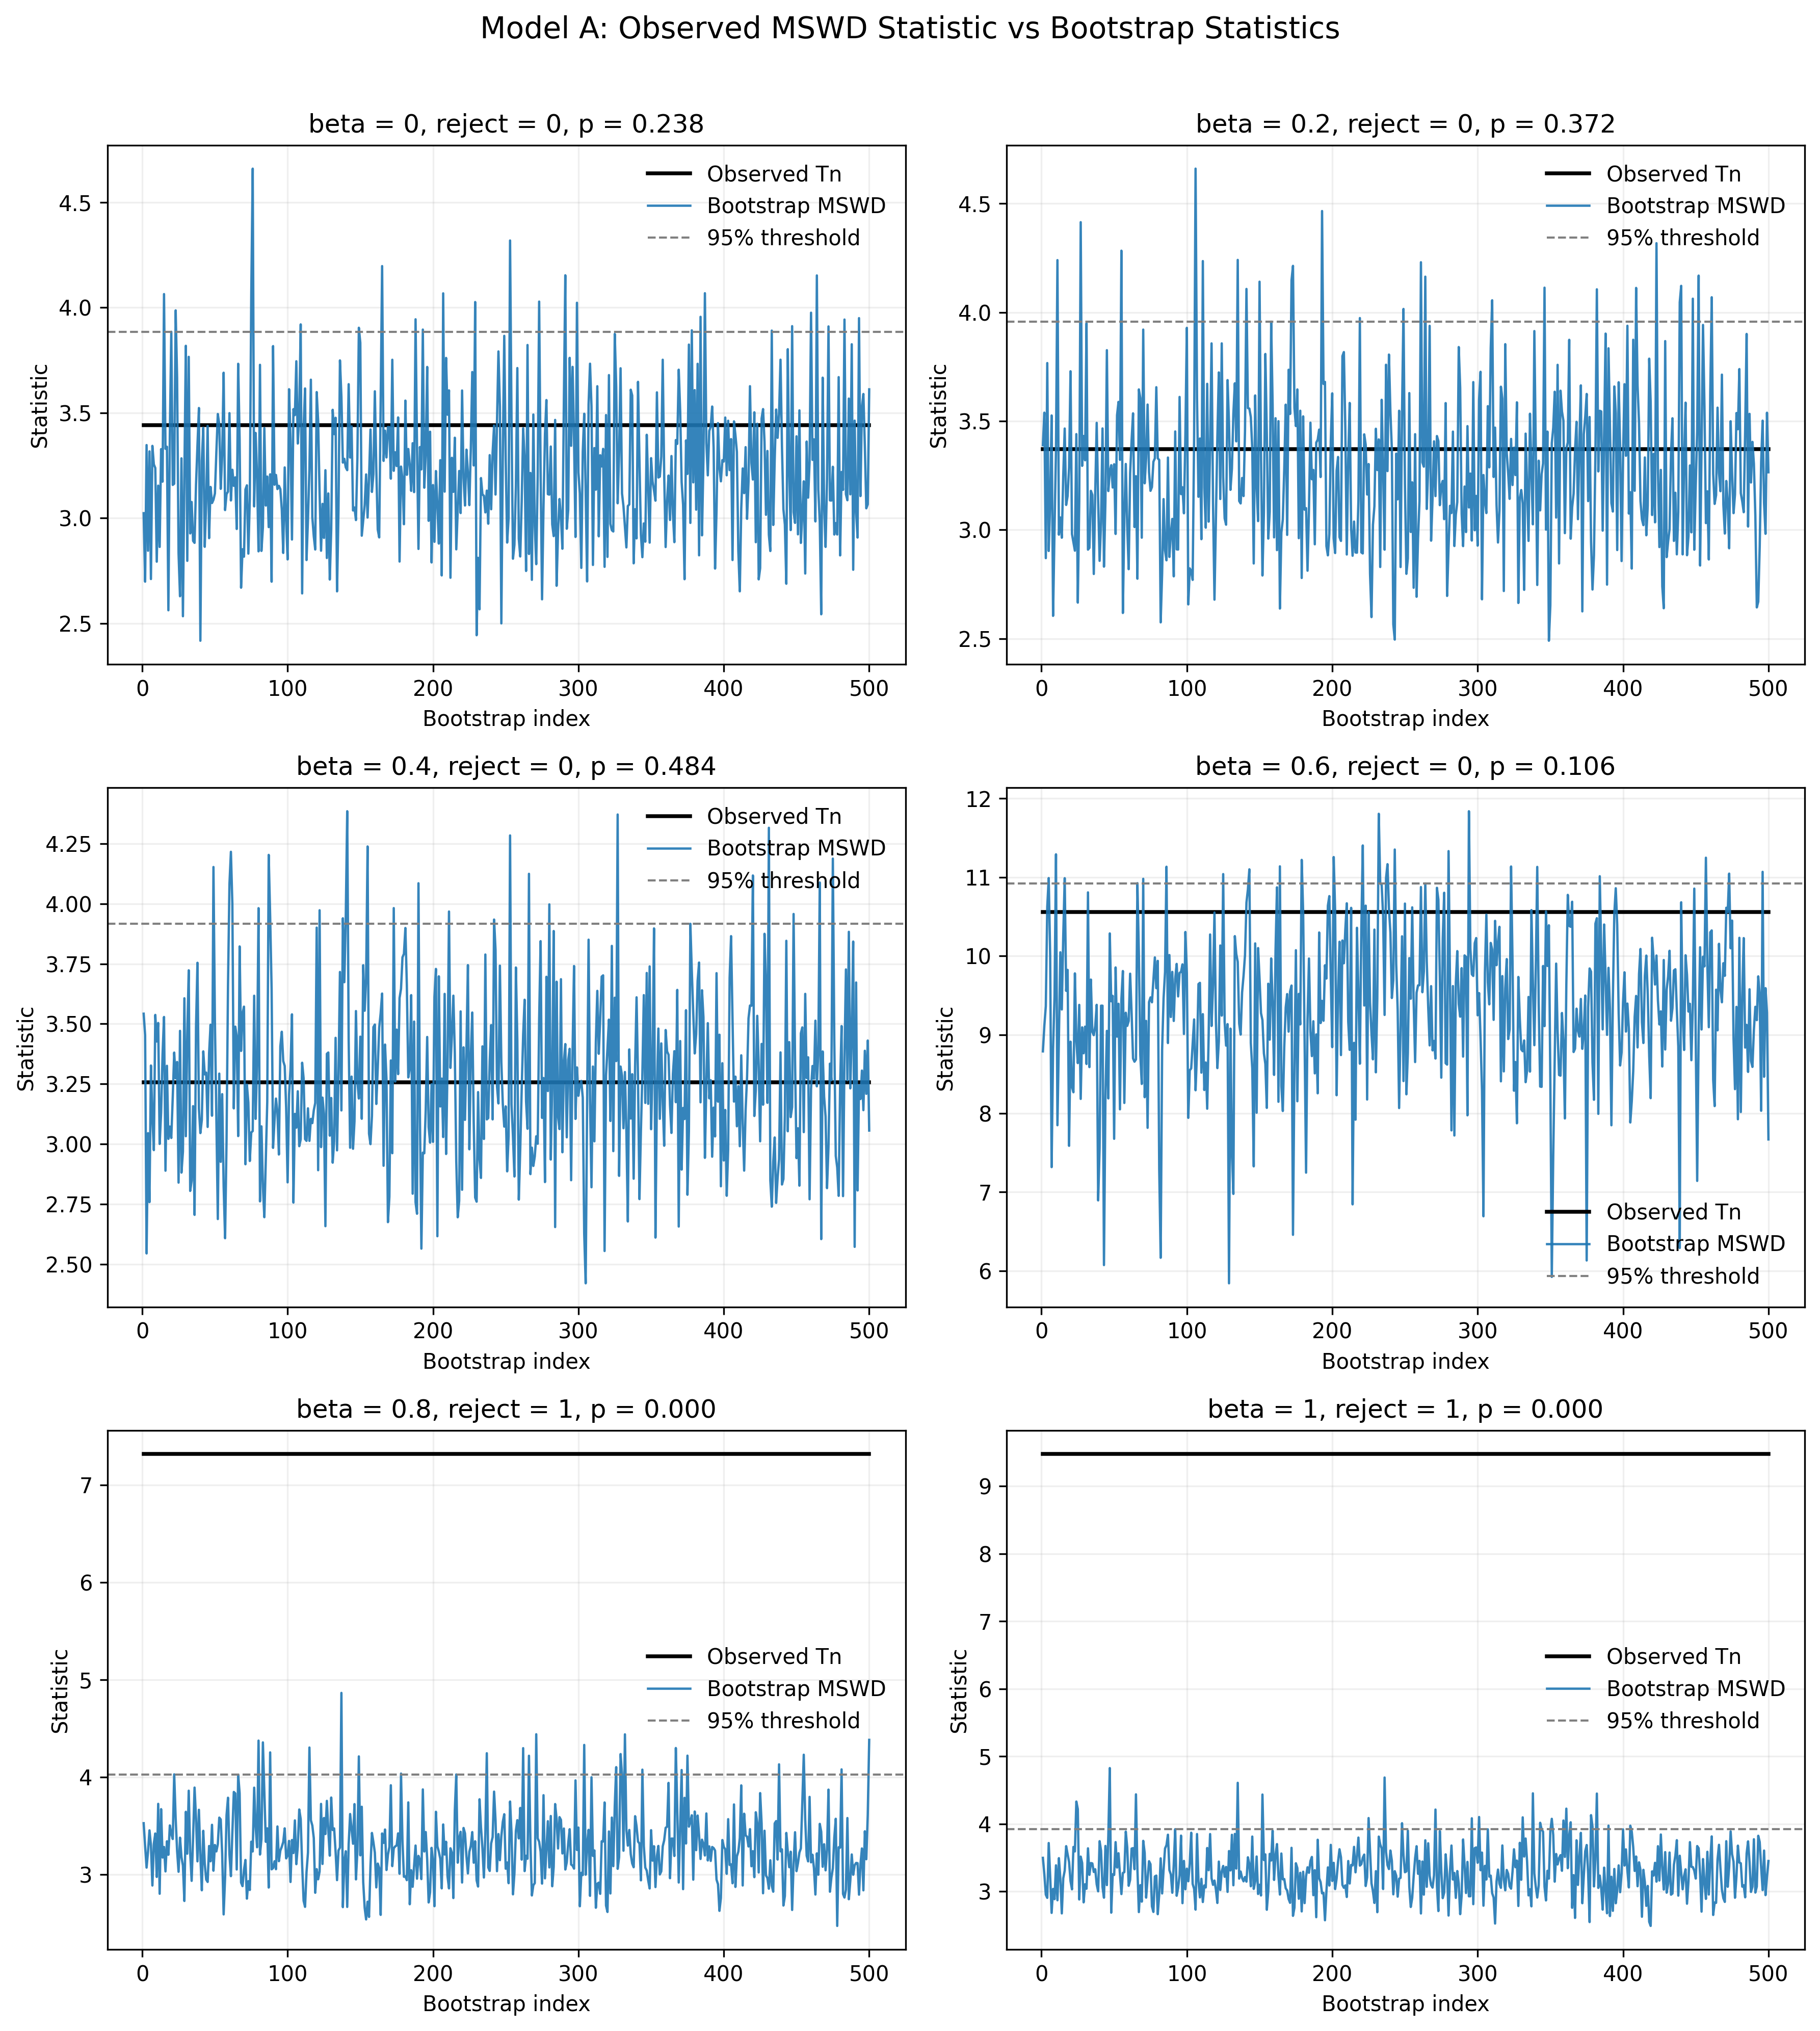
\includegraphics[width=0.84\linewidth,height=0.74\textheight,keepaspectratio]{fig2.png}
\end{center}
\end{frame}

\begin{frame}{Experiment 2 interpretation}
\small
\begin{tabular}{ccccc}
\toprule
\(\beta\) & observed \(T_n\) & threshold & p-value & reject \\
\midrule
0.0 & 3.442 & 3.885 & 0.238 & no \\
0.2 & 3.372 & 3.958 & 0.372 & no \\
0.4 & 3.256 & 3.918 & 0.484 & no \\
0.6 & 10.557 & 10.920 & 0.106 & no \\
0.8 & 7.319 & 4.025 & 0.000 & yes \\
1.0 & 9.479 & 3.921 & 0.000 & yes \\
\bottomrule
\end{tabular}

\vspace{0.25cm}
\begin{itemize}
  \item \(\beta=0.6\) is a borderline non-rejection in this single draw.
  \item A zero empirical p-value with 500 bootstraps should be reported as \(p<0.002\).
\end{itemize}
\end{frame}

\begin{frame}{Experiment 3 setup: LGG/GBM DNA methylation}
\begin{itemize}
  \item Data: TCGA LGG and GBM DNA methylation.
  \item Samples: \(n_1=511\) LGG and \(n_2=150\) GBM.
  \item Features: \(p=207\) glioma prognosis-related genes.
  \item Method: L0 sparse MSWD + bootstrap, \(B=500\), \(\alpha=0.05\).
  \item Aim: test global distributional equality and localize the differences.
\end{itemize}
\end{frame}

\begin{frame}{Experiment 3 global result: LGG differs from GBM}
\begin{tabular}{lc}
\toprule
Metric & Value \\
\midrule
Test statistic & 42.9236 \\
Bootstrap critical value & 1.8479 \\
Empirical p-value & \(p<0.002\) \\
Significant marginal genes & 138 / 207 \\
Significant GO terms & 7 / 7 \\
\bottomrule
\end{tabular}

\vspace{0.5cm}
\begin{itemize}
  \item The global statistic is far above the critical value.
  \item The paper reports 139 significant marginal genes; this reproduction finds 138.
\end{itemize}
\end{frame}

\begin{frame}{Experiment 3 GO-term result}
\begin{tabular}{lcc}
\toprule
GO term & Genes & Statistic \\
\midrule
mitotic cell cycle & 5 & 9.467 \\
mitotic cell cycle process & 4 & 9.465 \\
cell cycle process & 7 & 10.196 \\
cell cycle & 11 & 15.454 \\
DNA metabolic process & 6 & 8.730 \\
cell division & 5 & 11.126 \\
mitotic nuclear division & 3 & 4.131 \\
\bottomrule
\end{tabular}

\vspace{0.4cm}
All seven subsets are significant, concentrating the difference in cell-cycle, DNA-metabolic, cell-division, and mitotic processes.
\end{frame}

\begin{frame}{Experiment 3 QQ plots: projected distributions depart visibly}
\begin{center}
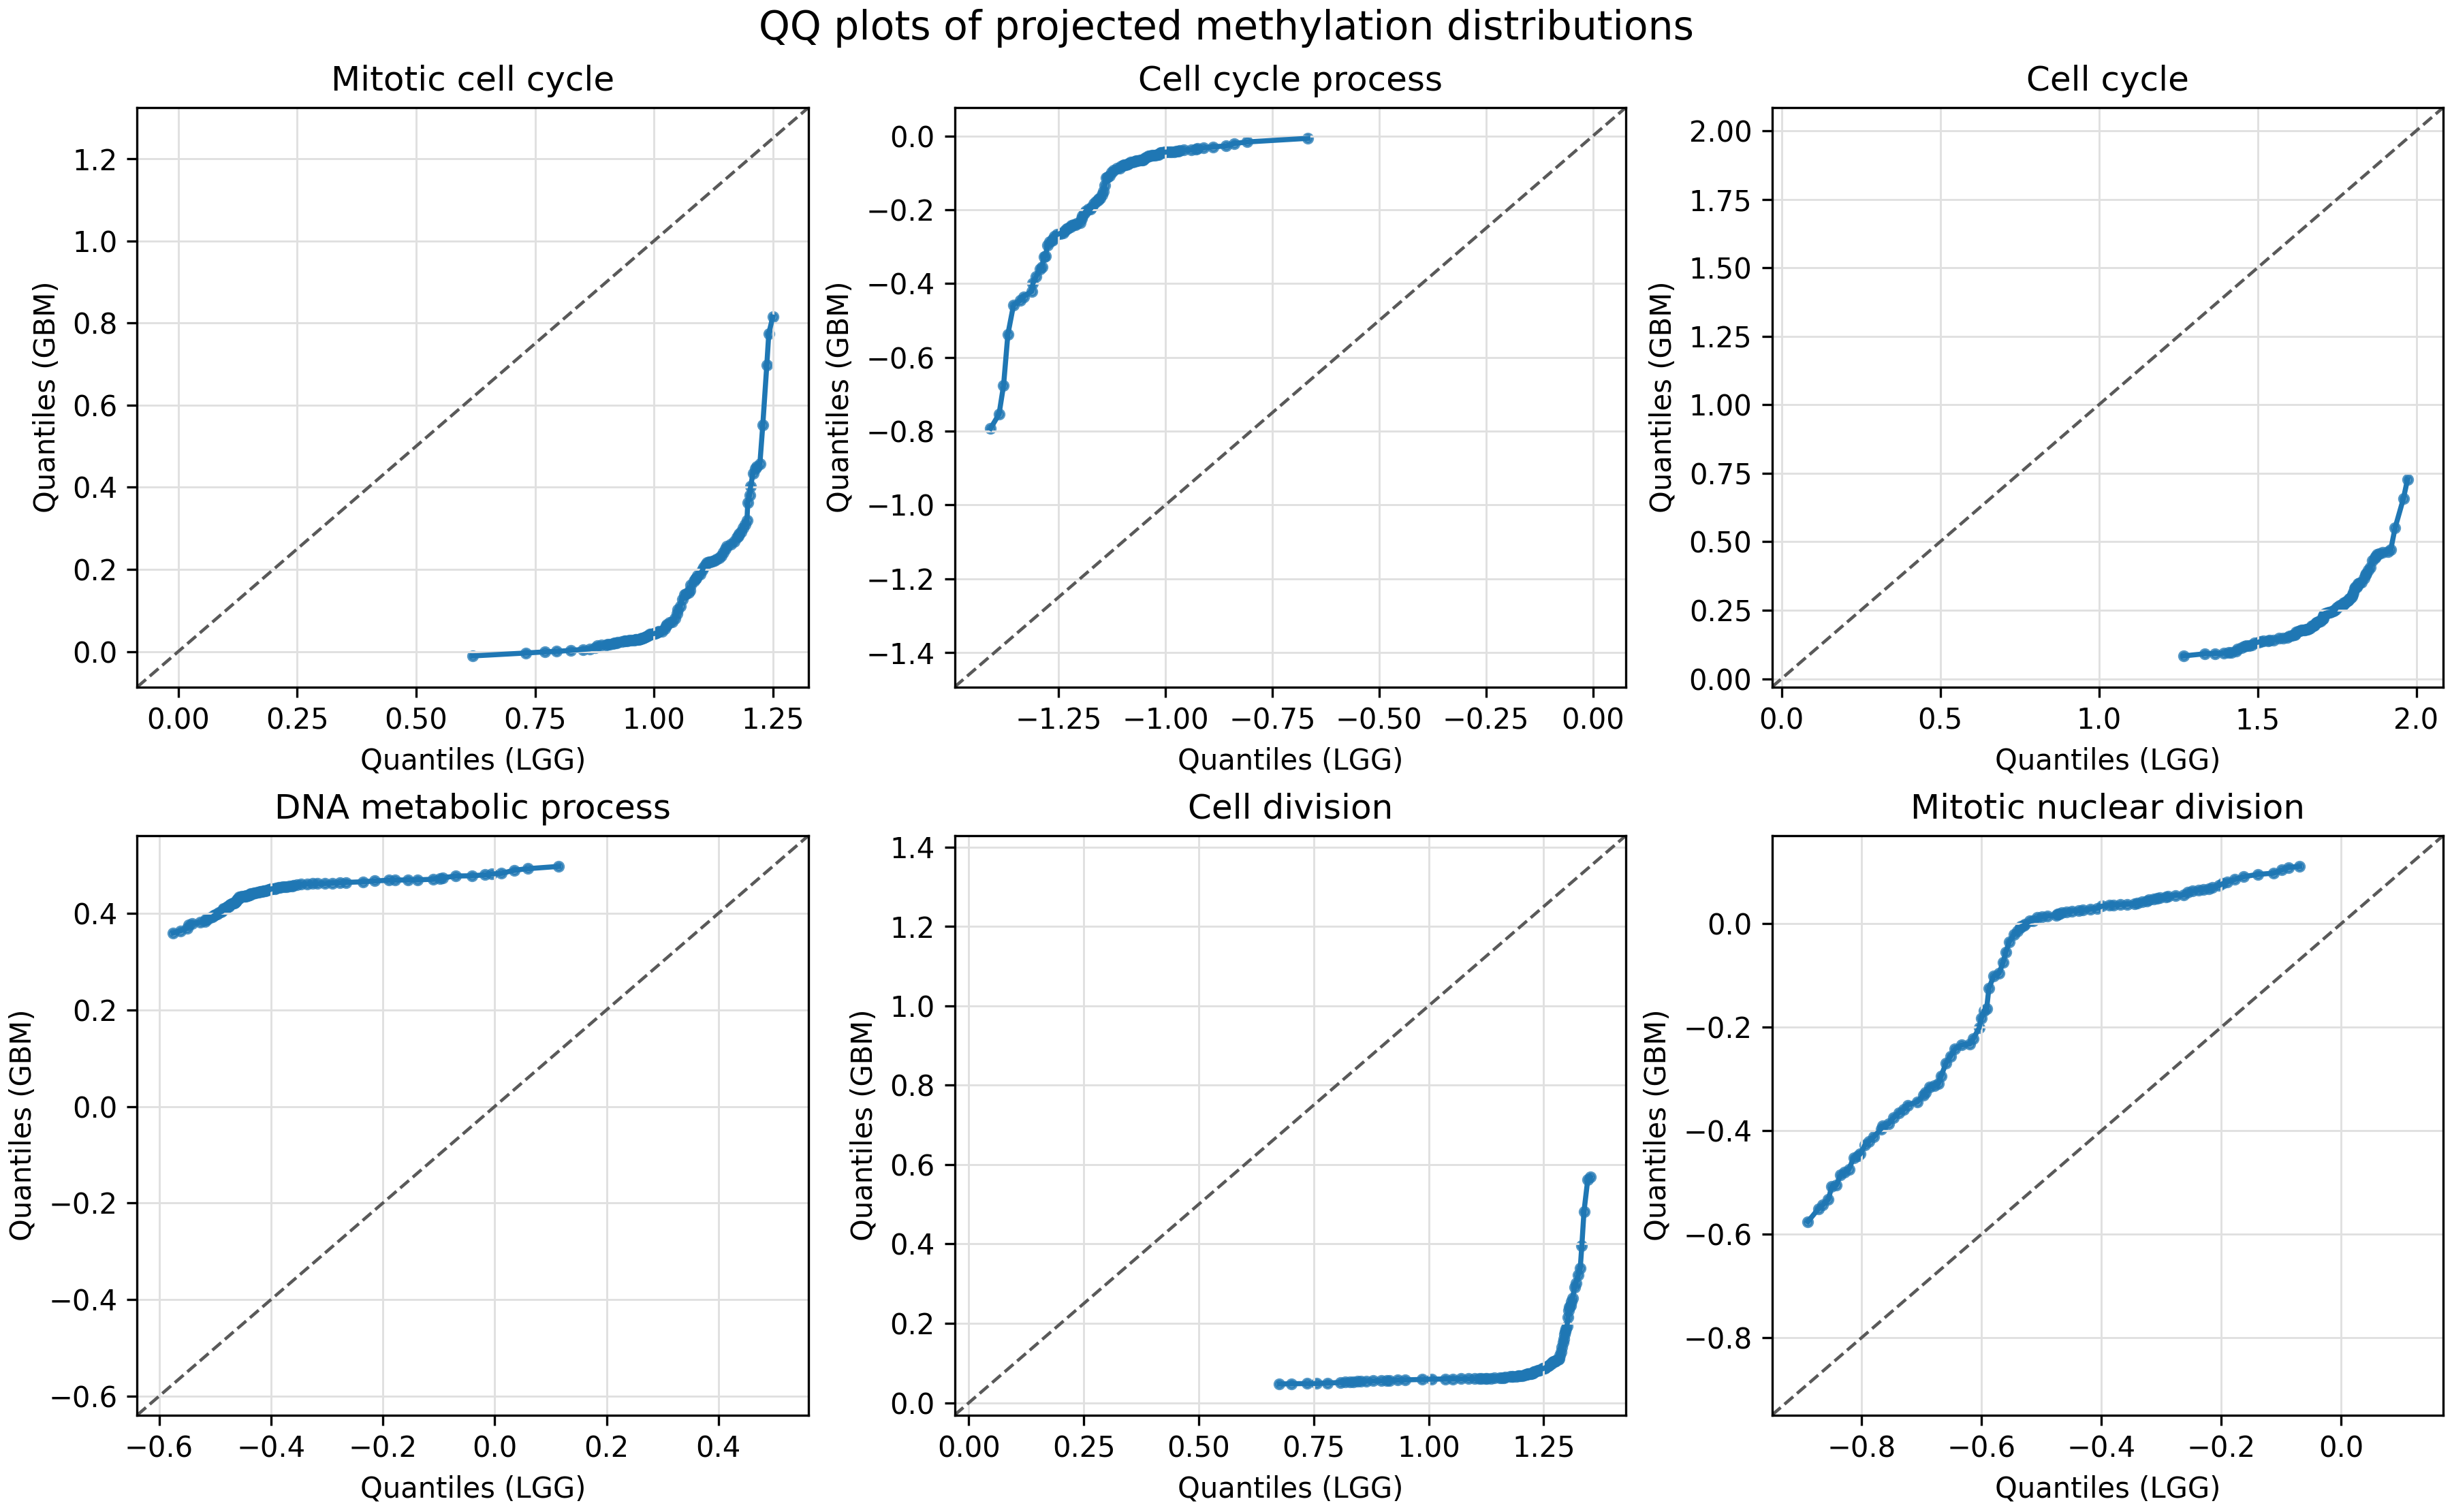
\includegraphics[width=0.82\linewidth,height=0.74\textheight,keepaspectratio]{fig3.png}
\end{center}
\end{frame}

\begin{frame}{Integrated conclusion}
\small
\begin{itemize}
  \item Experiment 1: MSWD has the strongest power under sparse decaying mean shifts.
  \item Experiment 2: bootstrap thresholds explain the Proposed method's rejection decision.
  \item Experiment 3: real GBM data show significant differences globally, marginally, and at the GO-term level.
  \item Methodological reason: max-sliced search reduces signal dilution, and SCI unifies testing with localization.
\end{itemize}
\end{frame}

\end{document}
